% Diese Zeile bitte -nicht- aendern.
\documentclass[course=asp]{aspdoc}

%newly added packages
\usepackage{microtype}
\usepackage{graphicx}
\usepackage{wrapfig}
\usepackage{enumitem}
\usepackage{amssymb}
\usepackage{amsthm}
\usepackage{listings}

\usepackage{amsmath}	%eins von beidem?
\usepackage{mathtools}

\usepackage{index}

%%%%%%%%%%%%%%%%%%%%%%%%%%%%%%%%%
%% TODO: Ersetzen Sie in den folgenden Zeilen die entsprechenden -Texte-
%% mit den richtigen Werten.
\newcommand{\theGroup}{132} % Beispiel: 42
\newcommand{\theNumber}{A214} % Beispiel: A123
\author{Mohammed Attia \and Patrick Zimmermann \and Thomas Torggler}
\date{Wintersemester 2020/21} % Beispiel: Wintersemester 2019/20
%%%%%%%%%%%%%%%%%%%%%%%%%%%%%%%%%

% Diese Zeile bitte -nicht- aendern.
\title{Gruppe \theGroup{} -- Abgabe zu Aufgabe \theNumber}

\begin{document}
\maketitle

\newpage
\section{Einleitung}

Raumf\"ullende Kurven bilden eine Br\"ucke zwischen Kunst und mathematischer Geometrie. In der Mathematik werden sie gemeinhin benutzt um ein $n$-dimensionales Problem in ein eindimensionales zu konvertieren. Eine solche Kurve beschreibt essentiell einen linearen Pfad durch $n$-dimensionale R\"aume. Giuseppe Peano war der Erste, der eine solche Kurve 1890 definierte.

Um einen n-dimensionalen Raum in die Dimension n-1 zu konvertieren, l\"asst sich eine stetig surrjektive Funktion $f(x)$ erstellen, so das gilt: $\forall x \in \mathbb{R}^{n-1} \quad \exists y \in \mathbb{R}^n$. F\"ur einen Beweis siehe (QUELLE?). Hier wollen wir uns auf die sogenannten Peano-Kurven beschr\"anken. F\"ur eine solche Kurve definieren wir ein Intervall $I = [0;1]$, sowie  $f: I \rightarrow I^2 $. Dann ist die Peano-Kurve: $\lim\limits_{x \to \infty}f(x)$, mit $x \in I$. Sie \{ entspricht dem Grenzwert einer Folge von Funktionen f(x) und \} l\"asst sich mit der Bedingung, dass sich die Kurve nicht \"uberschneiden darf, folgendermaßen konstruieren:

Man unterteile eine Fl\"ache in 9 Quadrate. Jedes dieser Quadrate soll nun durch eine Kurve besucht werden. Dadurch durchl\"auft die Kurve die Quadrate in Form eines „S“.
In einem Iterationsschritt l\"asst sich eines der 9 Quadrate in weitere 9 Quadrate Unterteilen, die wiederum auf selbe Art verbunden werden, wie in Abb.1 gezeigt.

\begin{figure} [ht] %vorher, eigentlich bild unter text
\centering
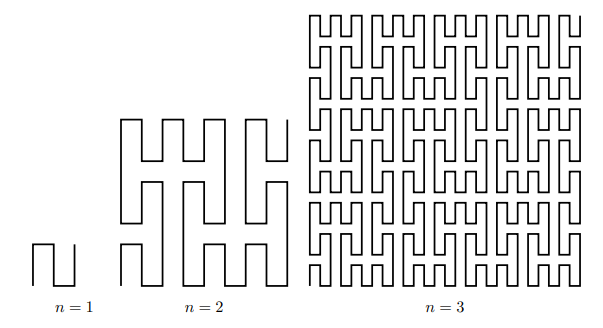
\includegraphics{PeanoBsp.png}
\caption{Peano-Kurve mit n = \{1, 2, 3\}, ~\cite{aufgabenstellung}}\label{Abb:Peano}	
\end{figure}

Im Folgenden Definieren wir $n \in \mathbb{N}$ als Grad der Kurve.
Wir beschreiben nun unseren Ansatz einen iterativen Algorithmus mit dem Grad $n$ als Eingabe zu finden, um die eben beschriebene Peano-Kurve darzustellen. Die hierbei generierten Punkte werden in ihrer Reihenfolge ausgegeben. Anders als in der beschriebenen mathematischen Definition werden wir jedoch nicht nur nach $[0;1]$ sonder nach $\mathbb{N}$ abbilden.

%Ergebnis hier einf\"ugen!! dann ist auch das Format besser

\newpage

\section{L\"osungsansatz}
Der Aufbau der Peano-Kurve erm\"oglicht es die Kurve des aktuellen Grades mit einer Variation der gespiegelten und originalen Kurve des vorherigen Grades zu zeichnen.
Diese Observation war der Grundstein unseres iterativen Algorithmus. Anfangs wird dabei die Startkurve hardcodiert in einem Integer Array abgespeichert wobei die Zahlen von 0 bis 3 jeweils einer der vier Richtungen entsprechen. Falls der eingegebene Grad $n > 1$ ist, wird aufsteigend \"uber alle Grade bis inklusive n iteriert wobei w\"ahrend jedem Schritt die Kurve des vorherigen Grades in der originalen Reihenfolge des ersten Grades entweder im Originalzustand oder gespiegelt acht mal in den Array eingef\"ugt wird, sodass die vollst\"andige Kurve des aktuellen Grades entsteht. 

\begin{figure}[ht]
\centering
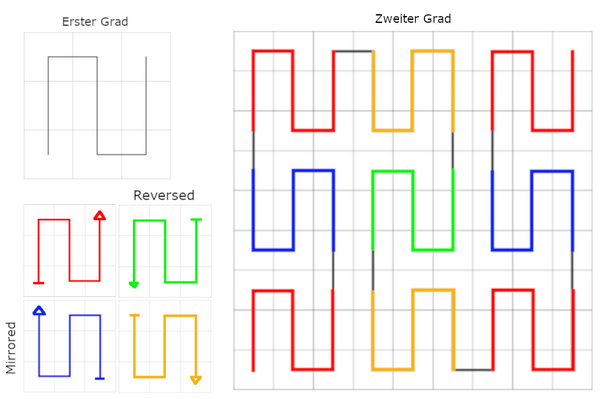
\includegraphics[scale=0.4]{PeanoFarbcodiert.png}
\caption{Peano-Kurve mit n = 1, n = 2}\label{Abb:Peano L\"osungsidee}
\end{figure}

Zu beachten ist dabei jedoch, dass durch das Spiegeln und Einf\"ugen von Kurven deren Richtung noch inkorrekt sein k\"onnte, daf\"ur gibt es aber \"ahnlich zur Spiegelungsmethode eine Methode zum Umkehren der Richtung. Nach diesen Schritten sind die neun erstellten Kurven jedoch noch nicht miteinander verbunden. Da sich das Muster der urspr\"unglichen Kurve durch alle Grade wiederholt, kann nach jedem Schritt ein hardcodierter Pfad zur n\"achsten Kurve eingef\"ugt werden.
Nachdem \"uber alle Grade iteriert wurde, l\"auft der Algorithmus den vollst\"andigen Richtung Array durch, ver\"andert dabei bei jedem Schritt je nach Richtungsangabe entweder die x oder y-Koordinate und speichert diese dann in die Ausgabeliste der Peano-Methode.

\newpage

\section{Korrektheit} % oder Genauigkeit

% Beweisen, dass nichts anderes als die gew\"unschten Permutationen entstehen!!

Die Genauigkeit unseres Algorithmus ist abh\"angig von dem Grad $n$, dass die Anzahl an Iterationen bestimmt, wie in den Abb.1 beschrieben. Das geht auch aus der beschriebenen mathematischen Definition hervor, da die Peano-Kurve an sich ein Grenzwert ist. Somit wird der Algorithmus genauer, je gr\"oßer der Grad der Kurve ist, da die Punkte auf der Kurve sich ebenfalls einem Grenzwert ann\"ahern. Ansonsten ist die Kurve wie ebenfalls schon oben beschrieben definiert, weshalb nun die Korrektheit unseres Algorithmus entscheidend ist.
Grunds\"atzlich l\"asst sich die Korrektheit einer Kurve, besonders bei der von uns behandelten, nachweisen indem man ihre graphischen Darstellungen vergleicht. Da das Theoretisch aber nicht m\"oglich ist, folgt auch eine Implementierung in Assambler und in C, die wir auch hinsichtlich ihrer Performanz analysieren wollen.
Wir wollen dennoch unseren Ansatz auf Korrektheit pr\"ufen.

\subsection{Beweis der Permutationen durch Induktion}
Nachdem die Kurve immer wieder die gleichen, teilweise elementaren, Bestandteile verwendet, m\"ussen diese und deren Permutationen richtig berechnet werden. Im speziellen sind das die Kurven mit $n = 1$ und $n = 2$. Aus diesen l\"asst sich induktiv die Korrektheit beweisen, da wir, wie im vorherigen Kapitel beschrieben, zum berechnen eine Kurve $n$-ten Grades nur die Kurve des Grads $n - 1$ sowie die gespiegelte und invertierte Version dieser benutzen. Bei der als invertierten Version betitelten Permutation handelt es sich in diesem Kontext um eine Punktspiegelung im Mittelpunkt der vorhergehenden Kurve, siehe Abb.2, weitere Erl\"auterungen folgen.	%echt Punktsymetrisch?

\subsubsection{Induktionsbasis}
Beginnen wir mit $n = 1$. Hier ist die Kurve vordefiniert, dementsprechend gibt es nichts zu zeigen. Da auf diesem Muster alle anderen Kurven mit $n > 1$ basieren, ist sie in unserem Algorithmus ebenfalls als Basis fest gegeben.
Des Weiteren ist die Definition der Kurve mit $n = 2$ f\"ur die Berechnung aller weiteren Kurven von N\"oten, da man anhand dieser Kurve alle notwendigen Bedingungen der Konstruktion weiterer Kurven ableiten kann. Deshalb nehmen wir sie also auch als definiert an \cite{aufgabenstellung}. Diese Bedingungen sollen im folgenden ebenfalls gepr\"uft werden.

\subsubsection{Induktionsannahme}
Da die Funktion wie vorher definiert surrjektiv ist, gilt:

\begin{center}
$\forall n > 1 \in \mathbb{N}$, $\exists y \in \mathbb{R}^n$ mit $x \in [0,1]$: $f(x)= y$	%evtl \"andern...
\end{center}

Dadurch lassen sich Kurven mit h\"oherem Grad konstruieren. Sei nun $n > 1$ und beliebig gew\"ahlt.

\subsubsection{Induktionsschritt}
Betrachten wir nun Kurven $n$-ten Grades. Hierzu m\"ussen wir die Permutationen der vorhergehenden Kurve untersuchen, die wir zur Konstruktion der Kurve mit Grad n ben\"otigen.	

%Invertierung - Reverse in Implementierung
Die invertierte Permutation ist im Kern nichts anderes als die normale Peano-Kurve mit anderer Reihenfolge der Koordinatenberechnung, im speziellen von $p_1=(1,1)$ nach $p_2 = (0,0)$. Dies hat zur Folge, dass sich außer der Reihenfolge der Punkte an der grundlegenden Kurve nichts \"andert. Somit ist die Invertierte Permutation induktiv eben so korrekt wie die zugrundeliegende Kurve niedrigeren Grades, siehe auch Abb.2, gr\"une Kurve.

%Spiegelung - Mirror in Implementierung
Bei der Spiegelung wird die Kurve an der Y-Achse gespiegelt. Wir ver\"andern also ebenfalls die vertikale Richtung, behalten jedoch weiterhin die horizontale Richtung bei. Dadurch wird die vorausgehende Kurve notwendiger weise ver\"andert. Diese zus\"atzliche Operation ist elementar und hat somit nur direkt auf die Koordinatenberechnung Einfluss, ohne die Kurve anderweitig zu ver\"andern und \"andert so den charakteristischen Verlauf der Kurve nicht. Siehe auch Abb.2, gelbe Kurve.

%Kombination von beidem
Abschließend bleibt noch die Kombination aus der vorangehenden Permutationen, die ebenfalls f\"ur die Konstruktion der Kurve von N\"oten ist. 


%Verbinden der Permutationen
Die unterschiedlichen Permutationen der Peano-Kurve werden durch eine eben solche Kurve mit $n = 1$ verbunden. Dadurch bleiben alle Eigenschaften der Kurve erhalten, da wir keine weiteren Punkte in die Kurve einf\"ugen, sonder nur die Art der graphischen Darstellung. Zudem ist dies auch ebenso Teil der Definition dieser Kurve. 

%Mathematischen sachen be/ver-weisen!
%Punktsymetrie egal!

\newpage
\section{Performanzanalyse}
Bevor den bereits ausgef\"uhrten Algorithmen hinsichtlich seiner Performanz analysieren, beschreiben wir nun kurz die Algorithmen, die wir zu den Vergleichen heranziehen.

Als erstes implementierten wir den bereits erl\"auterten Algorithmus aus dem Kapitel  \textit{L\"osungsansatz} in C implementiert. Um die Performanz-Unterschiede zwischen der direkten Berechnung, im Weiteren als Inplace-Variante, und der einmaligen Berechnung und Speicherung der Permutationen, im Folgenden als Out-Of-Place-Variante bezeichnet, erweitern wir die Implementation um einen Entsprechenden Algorithmus, welcher eine Abgewandelte Form der Inplace-Variante ist. Der Unterschied besteht darin, dass sobald wir eine Kurve mit $n > 2$ berechnen speichern wir uns die schon vorher besprochenen Permutationen der Kurve mit Grad $n - 1$.

\subsection{Technische Limitationen} %in C
Bei dem testen unseres Programms fallen bei Graden von $n > 6$ bestimmte technische Limitationen unser Rechensysteme auf. 

Zum einen haben wir kein Programm gefunden, dass die generierten .svg Dateien von einer Gr\"oße 43.0 Megabyte (Peano-Kurve mit $n = 7$) \"offnen kann. Mit zunehmendem Grad enth\"alt die .svg Dateien logischerweise immer mehr Punkte der Kurve, weshalb sie ebenfalls exponentiell zur Basis 9 steigt. Deshalb m\"ochten wir an dieser Stelle auf das Kapitel \textit{Korrektheit} verweisen um die Kurve auf selbige zu pr\"ufen.

Zum anderen ist es nicht m\"oglich, beliebig viel Speicher zu allokieren, da die von uns benutzte \textit{malloc}-Funktion maximal 17.179.869.184 Bytes auf dem Heap allokieren kann und der Heap zus\"atzlich in seiner Gr\"oße begrenzt ist. Deshalb k\"onnen wir auf unseren Systemen die Funktion mit maximal $n = 9$ ausf\"uhren, da sonst nicht gen\"ugend Speicher allokiert wird. F\"ur $n = 10$ m\"ussten 27.894.275.208 Bytes allokieren, wozu wir eben nicht im Stande sind, weshalb wir den Wertebereich von $n$ auf $[1;9]$ limitiert haben.

Um zu ermitteln, wie viel Speicher wir allokieren k\"onnen, haben wir eine For-Schleife  folgenden Typs ausgef\"uhrt:


\begin{lstlisting} %Formatieren! 
u\_int64\_t *v;    	
for (u\_int64\_t i = 1; v = (u\_int64\_t *) malloc(i); i <<= 1)   
\{     
print(i);
free(v); 
\}
\end{lstlisting}

%Assembler 


\newpage
\section{Zusammenfassung und Ausblick}

% TODO: Fuegen Sie Ihre Quellen der Datei Ausarbeitung.bib hinzu			!!!!
% Referenzieren Sie diese dann mit \cite{}.									
% Beispiel: CR2 ist ein Register der x86-Architektur~\cite{intel2017man}.
\bibliographystyle{plain}
\bibliography{Ausarbeitung}{}

\end{document}
